\chapter{Tasa de Cambio Relativa Óptima Conmutada y sus Variantes}
\label{cap:tcroc}

% -------------------------------------------------------------------
% Introducción

% --- SECCIÓN: Introducción y Motivación Matemática ---
\section{Introducción y Motivación Matemática}
\label{sec:tcroc_introduccion}

El análisis riguroso de fenómenos económicos modelados mediante Cadenas de Markov Ocultas (HMM) o procesos estocásticos de salto de régimen (Markov-Switching) requiere que el espacio de estados subyacente refleje transiciones dinámicas estacionarias o localmente estables. No obstante, las series temporales en finanzas y economía suelen ser altamente no estacionarias y dominadas por ruido. 

En este capítulo se cimenta la base matemática requerida para preparar y transformar la serie temporal cruda antes de someterla a cualquier proceso riguroso de \textbf{discretización de estados}. Se desarrolla formalmente la familia de transformaciones denominada \textbf{Tasa de Cambio Relativa Óptima Conmutada (TCROC)} y sus tres variantes operacionales: la \textbf{TCROCM} (con ventana móvil), la \textbf{ETCROC} (con decaimiento exponencial) y su forma general \textbf{ETCROCM} (con decaimiento exponencial y ventana móvil).

El objetivo de este capítulo es demostrar que el operador TCROC transforma una serie en tiempo discreto $\{v(t)\}_{t=0}^T$ en una secuencia continua de tasas de cambio $\{\alpha_t\}$ mediante la minimización convexa de $v(t) \approx (1+\alpha_t)v(t-1)$. Se demuestra que esta transformación satisface existencia, unicidad, continuidad y estabilidad frente a perturbaciones, propiedades necesarias para que la posterior discretización mediante K-Means produzca agrupaciones consistentes y evite asignaciones de régimen espurias.

Todas las variantes admiten solución analítica cerrada y tienen menor complejidad computacional que métodos iterativos como la máxima verosimilitud en MS-AR. Este capítulo constituye el primer bloque teórico de la tesis: se presentan los teoremas, lemas y demostraciones de consistencia que fundamentan el operador.

% Axiomática del Operador

% --- SECCIÓN: Axiomática del Operador de Tasa de Cambio Local ---
\section{Axiomática del Operador de Tasa de Cambio Local}
\label{sec:tcroc_axiomas}

Para que la transformación $\mathcal{T}: \mathbb{R}^{T+1} \to \mathbb{R}^T$ que genera la secuencia $\{\alpha_t\}$ sea compatible con una posterior discretización en cadena de Markov, debe satisfacer un conjunto mínimo de propiedades algebraicas y analíticas. La familia TCROC se construye de modo que cumpla los siguientes cuatro axiomas:

\begin{description}
    \item[Axioma 1 (Localidad Acotada y Dependencia Estricta):]
    El estado continuo de la tasa de cambio en un instante $t$,
    denotado como $\alpha_t$, depende exclusivamente de un
    subconjunto cerrado del pasado inmediato $[t-W+1, t]$.  Esta
    dependencia captura la dinámica inercial de los mercados y
    rechaza la influencia de estados temporales infinitamente
    lejanos.
    \item[Axioma 2 (Proporcionalidad Geométrica Local):] La relación entre valores consecutivos se modela como $v(t) = \beta_t\, v(t-1) + \varepsilon_t$. La tasa de cambio $\alpha_t = \beta_t - 1$ representa la variación relativa local entre observaciones adyacentes.
    \item[Axioma 3 (Unicidad y Convexidad Global):] El escalar $\alpha_t$ se obtiene como el mínimo global de una funcional de costo estrictamente convexa en $L^2$, lo que garantiza unicidad de la solución.
    \item[Axioma 4 (Estabilidad de Lipschitz frente a Perturbaciones):]
    Existe una constante $C > 0$ tal que variaciones acotadas en la
    serie observada $\|v' - v\|_\infty \leq \epsilon$ inducen
    desviaciones finitamente controladas en la proyección:
    \[
    |\alpha' - \alpha| \leq C\epsilon,
    \]
    lo que garantiza que la discretización posterior sea robusta ante ruido en los datos.
\end{description}

A lo largo de este capítulo se demostrará matemáticamente que las diferentes instanciaciones del modelo base (TCROC, TCROCM, ETCROC y ETCROCM) satisfacen integralmente estos axiomas.

% --- SECCIÓN: Marco General Unificado ---
\section{Marco General Unificado}
\label{sec:tcroc_marco_general}

Sea \(T > 0\) un entero y \(\Sigma_T = \{v(0), v(1), \dots, v(T)\}\) una serie temporal con \(v(t) \in \mathbb{R}\). Dados un tamaño de ventana \(W\) con \(1 \leq W \leq T\) y un factor de decaimiento \(\lambda \in (0, 1]\), definimos para cada instante \(t \geq W\) la \textbf{tasa de cambio relativa óptima generalizada} como:

\begin{equation}
    \alpha_{t,\lambda,W} \;:=\; -1 + \arg\min_{\beta \in \mathbb{R}} \sum_{k=t-W+1}^{t} \lambda^{t-k} \bigl(v(k) - \beta\, v(k-1)\bigr)^2.
\label{eq:tcroc_general}
\end{equation}

Las cuatro variantes se recuperan como casos particulares:

\begin{center}
\renewcommand{\arraystretch}{1.3}
\begin{tabular}{lcc}
\toprule
\textbf{Variante} & \textbf{Parámetros} & \textbf{Notación} \\
\midrule
TCROC   & \(\lambda = 1,\; W = T\) & \(\alpha_T\) \\
TCROCM  & \(\lambda = 1,\; W < T\) & \(\alpha_{t}^{(W)}\) \\
ETCROC  & \(\lambda < 1,\; W = T\) & \(\alpha_{T,\lambda}\) \\
ETCROCM & \(\lambda < 1,\; W < T\) & \(\alpha_{t,\lambda,W}\) \\
\bottomrule
\end{tabular}
\end{center}

Esta estructura jerárquica se ilustra en la Figura~\ref{fig:jerarquia_tcroc}.

\begin{figure}[htbp]
    \centering
    \begin{tikzpicture}[
        node distance=1.5cm and 2.8cm,
        >=Stealth,
        % --- Estilos (mismos que Cap 5) ---
        base/.style={draw, rectangle, rounded corners=6pt, minimum width=3.2cm, 
                     minimum height=0.9cm, font=\small\bfseries, align=center,
                     drop shadow={shadow xshift=1pt, shadow yshift=-1pt, opacity=0.3}},
        canonical/.style={base, fill=nordSnow, draw=nordGray, text=nordDark},
        extension/.style={base, fill=nordSnow, draw=nordGray, text=nordDark},
        hybrid/.style={base, fill=nordSnow!80!nordFrost, draw=nordFrost, text=nordDark},
        edgelabel/.style={font=\scriptsize, fill=white, inner sep=2pt, opacity=0.9}
    ]

        % Nodos
        \node[canonical] (TCROC) {TCROC\\{\scriptsize $(W=T,\;\lambda=1)$}};
        
        \node[extension] (TCROCM) [below left=of TCROC] {TCROCM\\{\scriptsize $(W<T)$}};
        \node[extension] (ETCROC) [below right=of TCROC] {ETCROC\\{\scriptsize $(\lambda<1)$}};
        
        \node[hybrid] (ETCROCM) [below=2.8cm of TCROC] {ETCROCM\\{\scriptsize $(W<T,\;\lambda<1)$}};

        % Conexiones
        \draw[->, thick] (TCROC) -- (TCROCM) node[edgelabel, midway, left] {$+\,W$};
        \draw[->, thick] (TCROC) -- (ETCROC) node[edgelabel, midway, right] {$+\,\lambda$};
        \draw[->, thick] (TCROCM) -- (ETCROCM) node[edgelabel, midway, left] {$+\,\lambda$};
        \draw[->, thick] (ETCROC) -- (ETCROCM) node[edgelabel, midway, right] {$+\,W$};

        % Conexión directa (punteada)
        \draw[->, thick, dashed, nordGray!60] (TCROC) -- (ETCROCM)
            node[edgelabel, midway] {$(W, \lambda)$};

    \end{tikzpicture}
    \caption{Jerarquía paramétrica del operador TCROC y sus variantes. El nodo central representa la formulación global canónica ($W=T, \lambda=1$). La incorporación de memoria restringida ($W<T$) y decaimiento exponencial ($\lambda < 1$) producen las extensiones laterales, que convergen en el operador generalizado ETCROCM.}
    \label{fig:jerarquia_tcroc}
\end{figure}

% Propiedades Analíticas del Operador Generalizado

% --- SECCIÓN: Teoremas Fundamentales del Operador Generalizado ---
\section{Teoremas Fundamentales del Operador Generalizado}
\label{sec:tcroc_teoremas_generales}

Dado que la variante híbrida dinámica (ETCROCM) subsume paramétricamente a las formulaciones base (TCROC, TCROCM y ETCROC), se procede a demostrar las propiedades algebraicas, topológicas y asintóticas directamente sobre la forma generalizada \(\alpha_{t,\lambda,W}\) definida en la Ecuación \eqref{eq:tcroc_general}. Las demostraciones y garantías matemáticas para el resto de las variantes se infieren de manera colateral e inmediata por simple relajación o límite de parámetros.

Esta consolidación eleva el rigor analítico, demostrando que cualquier filtro derivado de esta familia cumple forzosamente con el comportamiento axiomático exigido previamente.

% --- SUBSECCIÓN: Existencia Ponderada y Unicidad Global --- - - - - - - - - - - - - - - - - - - - - - - - - - - - - - -
\subsection{Existencia Ponderada y Unicidad Global}
\label{subsec:teorema_existencia}

\begin{theorem}
\label{teo:existencia_general}
Para cualquier instante de tiempo válido \(t \geq W\), si el subconjunto de observaciones contenidas en la ventana local de rezagos exhibe al menos un suceso medible no nulo (formalmente, \(\exists k \in [t-W+1, t]\) tal que \(v(k-1) \neq 0\)), entonces la funcional de costo en el espacio topológico \(L^2\), definida como \(f(\beta) = \sum_{k=t-W+1}^{t} \lambda^{t-k} \bigl(v(k) - \beta\, v(k-1)\bigr)^2\), admite un y solo un minimizador global \(\hat{\beta}_{t,\lambda,W}\) formulado cerradamente por:
\begin{equation}
\hat{\beta}_{t,\lambda,W} = \frac{\displaystyle\sum_{k=t-W+1}^{t} \lambda^{t-k}\, v(k)\, v(k-1)}{\displaystyle\sum_{k=t-W+1}^{t} \lambda^{t-k}\, v(k-1)^2}.
\label{eq:beta_general}
\end{equation}
\end{theorem}

\begin{proof}
Sea $a = \sum_{k=t-W+1}^{t} \lambda^{t-k}\, v(k-1)^2$.  Dado que
$\lambda \in (0,1]$, cada peso $\lambda^{t-k}$ es estrictamente
positivo.  Por la hipótesis de no degeneración, existe al menos un
$k$ tal que $v(k-1) \neq 0$, de donde $a > 0$.  Entonces
$f(\beta) = a\beta^2 - 2b\beta + c$ con $a > 0$ es estrictamente
convexa y coerciva ($f(\beta) \to +\infty$ cuando
$|\beta| \to \infty$).  El mínimo global se alcanza en el único
punto donde $f'(\beta) = 2a\beta - 2b = 0$, es decir,
$\hat{\beta}_{t,\lambda,W} = b/a$, que coincide con la expresión
\eqref{eq:beta_general}.
\end{proof}

\begin{corollary}
\label{cor:etcrocm_alpha}
Bajo las mismas condiciones del Teorema~\ref{teo:existencia_general},
la tasa de cambio relativa
\begin{equation}
\alpha_{t,\lambda,W} = \hat{\beta}_{t,\lambda,W} - 1
\label{eq:alpha_general}
\end{equation}
está bien definida y es única para cada $t \geq W$.
\end{corollary}

Este resultado garantiza que los algoritmos de discretización
posteriores (e.g., K-Means) reciben una entrada bien definida,
evitando divisiones por cero o indeterminaciones numéricas.

% --- SUBSECCIÓN: Consistencia Asintótica Ergódica --- - - - - - - - - - - - - - - - - - - - - - - - - - - - - - -
\subsection{Consistencia Asintótica}
\label{subsec:teorema_consistencia}

\begin{theorem}[Consistencia del estimador]
\label{teo:consistencia_general}
Supóngase que la serie temporal $\{v(k)\}$ satisface localmente
el modelo autorregresivo de primer orden
$v(k) = \beta^* v(k-1) + \varepsilon_k$,
donde $\{\varepsilon_k\}$ es ruido blanco con
$\mathbb{E}[\varepsilon_k] = 0$ y
$\mathbb{E}[\varepsilon_k^2] = \sigma^2 < \infty$,
y $|\beta^*| < 1$ (estacionariedad).  Entonces, cuando
$W \to \infty$ con $\lambda \in (0,1]$ fijo,
\[
\hat{\beta}_{t,\lambda,W} \xrightarrow{p} \beta^*
\quad \text{y, en consecuencia,} \quad
\alpha_{t,\lambda,W} \xrightarrow{p} \beta^* - 1.
\]
\end{theorem}

\begin{proof}
Sustituyendo $v(k) = \beta^* v(k-1) + \varepsilon_k$ en la
expresión del estimador \eqref{eq:beta_general}, se obtiene
\[
\hat{\beta}_{t,\lambda,W}
= \frac{\sum_{k=t-W+1}^{t} \lambda^{t-k}
       (\beta^* v(k-1) + \varepsilon_k)\, v(k-1)}
      {\sum_{k=t-W+1}^{t} \lambda^{t-k}\, v(k-1)^2}
= \beta^* + \frac{N_W}{D_W},
\]
donde
$N_W = \sum_{k} \lambda^{t-k}\, \varepsilon_k\, v(k-1)$ y
$D_W = \sum_{k} \lambda^{t-k}\, v(k-1)^2$.

\textbf{Paso~1 (Denominador).}  Dado que $|\beta^*| < 1$, el proceso
$\{v(k)\}$ es estacionario y ergódico, con
$\mathbb{E}[v(k-1)^2] = \sigma^2/(1 - \beta^{*2}) > 0$.  Sea
$\Lambda_W = \sum_{k=t-W+1}^{t} \lambda^{t-k}$.  Por la Ley de los
Grandes Números para sucesiones ponderadas estacionarias
\cite{Anderson1971},
\[
\frac{D_W}{\Lambda_W} \xrightarrow{p}
\mathbb{E}[v(k-1)^2] = \frac{\sigma^2}{1 - \beta^{*2}} > 0.
\]

\textbf{Paso~2 (Numerador).}  Como $\varepsilon_k$ es independiente
de $\mathcal{F}_{k-1} = \sigma(v(0), \ldots, v(k-1))$, se tiene
$\mathbb{E}[\varepsilon_k v(k-1)] = 0$.  Por la desigualdad de Chebyshev,
\[
\text{Var}\!\left(\frac{N_W}{\Lambda_W}\right)
= \frac{\sum_{k} \lambda^{2(t-k)}\,
       \mathbb{E}[\varepsilon_k^2 v(k-1)^2]}{\Lambda_W^2}
\leq \frac{\sigma^2 \mathbb{E}[v(k-1)^2]
       \sum_{k} \lambda^{2(t-k)}}{\Lambda_W^2}
= \mathcal{O}\!\left(\frac{1}{W}\right) \to 0.
\]

\textbf{Paso~3 (Conclusión).}  Por el Lema de Slutsky,
$N_W / D_W = (N_W/\Lambda_W) / (D_W/\Lambda_W)
\xrightarrow{p} 0 / \mathbb{E}[v(k-1)^2] = 0$.
Por tanto, $\hat{\beta}_{t,\lambda,W} \xrightarrow{p} \beta^*$.
\end{proof}

\begin{remark}[Alcance de la hipótesis de estacionariedad]
\label{rem:estacionariedad}
La hipótesis $|\beta^*| < 1$ es esencial para la prueba, pues
garantiza que $\mathbb{E}[v(k-1)^2]$ sea finito.  Sin embargo, las
series económicas reales (como el PIB nominal) frecuentemente
exhiben tendencia, con $\beta^*$ cercano o igual a 1.  En tales
casos, el Teorema~\ref{teo:consistencia_general} no es directamente
aplicable a la serie $v(t)$ en niveles.

No obstante, el operador $\alpha_{t,\lambda,W}$ actúa como un
filtro de diferenciación local: $\alpha_t \approx v(t)/v(t-1) - 1$,
que es análogo a la tasa de crecimiento.  Para una serie con raíz
unitaria ($\beta^* = 1$), la serie de tasas
$\alpha_t = v(t)/v(t-1) - 1$ es generalmente estacionaria.  En la
implementación empírica, la consistencia se verifica por la
estacionariedad de $\{\alpha_t\}$, no necesariamente de $\{v(t)\}$.
La validación con tests ADF aplicados a la serie
$\{\alpha_t\}$ se presenta en el
Capítulo~\ref{cap:regimenes_combustibles}.
\end{remark}

% --- SUBSECCIÓN: Estabilidad de Lipschitz --- - - - - - - - - - - -
\subsection{Estabilidad de Lipschitz}
\label{subsec:teorema_estabilidad}

El Axioma~4 requiere que el operador sea robusto frente a
perturbaciones acotadas en los datos de entrada.  El siguiente lema
formaliza esta propiedad.

\begin{lemma}[Estabilidad tipo Lipschitz]
\label{lem:estabilidad_general}
Sean $\{v(k)\}$ y $\{v'(k)\}$ dos series tales que
$\|v' - v\|_\infty \leq \epsilon$ (perturbación uniforme acotada).
Defínase
$S_2 = \sum_{k=t-W+1}^{t} \lambda^{t-k}\, v(k-1)^2 > 0$.
Entonces
\[
|\alpha'_{t,\lambda,W} - \alpha_{t,\lambda,W}|
\leq C_t \cdot \epsilon,
\]
donde $C_t$ es una constante que depende de $v$, $\lambda$ y $W$,
satisfaciendo
$C_t = \mathcal{O}\!\bigl(\|v\|_{\ell^2} / S_2\bigr)$.
\end{lemma}

\begin{proof}
Sean $S_1 = \sum_k \omega_k\, v(k)v(k-1)$ y
$S_1' = \sum_k \omega_k\, v'(k)v'(k-1)$, con
$\omega_k = \lambda^{t-k}$.  Escribiendo $v'(k) = v(k) + \delta(k)$
con $|\delta(k)| \leq \epsilon$:
\begin{align*}
S_1' - S_1 &= \sum_k \omega_k\bigl[
  v(k)\delta(k-1) + \delta(k)v(k-1) + \delta(k)\delta(k-1)
\bigr].
\end{align*}
Por la desigualdad de Cauchy-Schwarz y la cota
$|\delta(k)| \leq \epsilon$:
\[
|S_1' - S_1| \leq 2\epsilon \sum_k \omega_k |v(k)| \cdot |v(k-1)|
+ \epsilon^2 \sum_k \omega_k
\leq 2\epsilon \Lambda_W \|v\|_{\ell^2}^2 / W + \epsilon^2 \Lambda_W.
\]
De manera análoga, $|S_2' - S_2| \leq
2\epsilon\sum_k \omega_k |v(k-1)| + \epsilon^2 \Lambda_W$.
Como $\alpha = S_1/S_2 - 1$, la diferencia
$|\alpha' - \alpha| = |S_1'/S_2' - S_1/S_2|$ se acota
mediante la fórmula del cociente:
\[
\left|\frac{S_1'}{S_2'} - \frac{S_1}{S_2}\right|
= \frac{|S_1' S_2 - S_1 S_2'|}{S_2 S_2'}
\leq \frac{S_2|S_1'-S_1| + |S_1||S_2'-S_2|}{S_2 S_2'}.
\]
Dado que $S_2' \geq S_2 - \mathcal{O}(\epsilon) > 0$ para
$\epsilon$ suficientemente pequeño, todos los términos del
numerador son lineales en $\epsilon$ (los cuadráticos en $\epsilon$
son de orden inferior), obteniéndose $|\alpha' - \alpha|
\leq C_t \epsilon$ con
$C_t = \mathcal{O}(\|v\|_{\ell^2} / S_2)$.
\end{proof}

% --- SUBSECCIÓN: Optimalidad de Gauss-Markov --- - - - - - - - - -
\subsection{Optimalidad de Gauss-Markov}
\label{subsec:teorema_optimalidad}

\begin{theorem}[Optimalidad GLS del estimador]
\label{teo:optimalidad_general}
Considérese el modelo lineal local
$v(k) = \beta\, v(k-1) + \varepsilon_k$ con errores
heterocedásticos cuya varianza decrece con la antigüedad:
$\mathrm{Var}(\varepsilon_k) = \sigma^2 / \lambda^{t-k}$,
donde $\lambda \in (0,1]$.  Entonces el estimador
$\hat{\beta}_{t,\lambda,W}$ definido en \eqref{eq:beta_general}
coincide con el \textbf{Estimador de Mínimos Cuadrados
Generalizados (GLS)} del modelo, y por el Teorema de
Gauss-Markov generalizado, es el estimador lineal insesgado de
mínima varianza (BLUE).
\end{theorem}

\begin{proof}
Bajo el modelo $\vect{v} = \beta\,\vect{v}_{-1} + \vect{\varepsilon}$
con $\mathrm{Cov}(\vect{\varepsilon}) = \sigma^2 \mat{\Omega}$,
donde $\mat{\Omega} = \mathrm{diag}(\lambda^{-(t-k)})_{k=t-W+1}^{t}$,
el estimador GLS es
\[
\hat{\beta}_{\text{GLS}}
= (\vect{v}_{-1}^T \mat{\Omega}^{-1} \vect{v}_{-1})^{-1}
  \vect{v}_{-1}^T \mat{\Omega}^{-1} \vect{v}.
\]
Como $\mat{\Omega}^{-1} = \mathrm{diag}(\lambda^{t-k})$, se tiene
\[
\hat{\beta}_{\text{GLS}}
= \frac{\sum_{k} \lambda^{t-k}\, v(k)\, v(k-1)}
      {\sum_{k} \lambda^{t-k}\, v(k-1)^2}
= \hat{\beta}_{t,\lambda,W},
\]
que coincide exactamente con el estimador ETCROCM.  La propiedad
BLUE se sigue del Teorema de Gauss-Markov generalizado
\cite{Aitken1936, Anderson1971}.
\end{proof}

% --- SECCIÓN: Casos Particulares del Estimador Generalizado ---
\section{Casos Particulares del Estimador Generalizado}
\label{sec:tcroc_corolarios}

Las variantes de la familia TCROC presentadas en la
Sección~\ref{sec:tcroc_introduccion} surgen como casos particulares
del estimador generalizado $\hat{\beta}_{t,\lambda,W}$ al
especializar los parámetros $W$ y $\lambda$.  A continuación se
formaliza cada variante como un corolario del
Teorema~\ref{teo:existencia_general}.

% --- SUBSECCIÓN: TCROC ---
\subsection{TCROC: Estimador Global
(\texorpdfstring{$W=T,\;\lambda=1$}{W=T, lambda=1})}

Al fijar $W = T$ y $\lambda = 1$, todos los pesos son unitarios
y la sumatoria abarca la totalidad de la serie.  El estimador se
reduce a
\begin{equation}
\hat{\beta}_T = \frac{\sum_{k=1}^{T} v(k)\, v(k-1)}
                    {\sum_{k=1}^{T} v(k-1)^2},
\qquad \alpha_T = \hat{\beta}_T - 1.
\label{eq:tcroc_global}
\end{equation}
Este estimador produce un escalar constante $\alpha_T$ que resume
la tendencia global de la serie.  Al no depender de $t$, sirve
como línea base (\textit{baseline}) contra la cual se comparan las
variantes locales.

\begin{remark}[Degeneración del TCROC global]
\label{rem:degeneracion_tcroc}
Dado que $\alpha_T$ es un escalar único para toda la serie, la
secuencia de estados discretos $S_t = \pi(\alpha_T)$ es constante:
todos los instantes se asignan al mismo régimen.  En consecuencia,
el modelo TCROC-Markov se vuelve trivial (la matriz de transición es
la identidad).  Esta degeneración se confirma empíricamente
en el Capítulo~\ref{cap:regimenes_combustibles}.  Por este
motivo, la variante TCROC ($W = T$, $\lambda = 1$) tiene un
rol exclusivamente teórico dentro de la jerarquía: sirve como
caso límite y línea base, pero en la práctica se emplean las
variantes locales (TCROCM, ETCROC, ETCROCM) con $W \ll T$.
\end{remark}

% --- SUBSECCIÓN: TCROCM ---
\subsection{TCROCM: Estimador con Ventana Móvil
(\texorpdfstring{$W<T,\;\lambda=1$}{W<T, lambda=1})}

Al restringir la ventana a $W < T$ pero manteniendo $\lambda = 1$
(pesos uniformes), el estimador utiliza únicamente las $W$
observaciones más recientes:
\begin{equation}
\hat{\beta}_{t}^{(W)} = \frac{\sum_{k=t-W+1}^{t} v(k)\, v(k-1)}
                            {\sum_{k=t-W+1}^{t} v(k-1)^2},
\qquad \alpha_t^{(W)} = \hat{\beta}_{t}^{(W)} - 1.
\label{eq:tcrocm}
\end{equation}
Esto produce una secuencia $\{\alpha_t^{(W)}\}_{t=W}^{T}$ que se
actualiza en cada instante, de manera análoga a una media móvil
autoregresiva.  La longitud $W$ controla el compromiso entre
sensibilidad local y estabilidad del estimador.

% --- SUBSECCIÓN: ETCROC ---
\subsection{ETCROC: Estimador con Decaimiento Exponencial
(\texorpdfstring{$W=T,\;\lambda<1$}{W=T, lambda<1})}

Al utilizar toda la muestra ($W = T$) pero con factor de
decaimiento $\lambda \in (0,1)$, las observaciones recientes
reciben mayor peso que las antiguas de forma geométrica:
\begin{equation}
\hat{\beta}_{T,\lambda} = \frac{\sum_{k=1}^{T} \lambda^{T-k}\,
  v(k)\, v(k-1)}{\sum_{k=1}^{T} \lambda^{T-k}\, v(k-1)^2},
\qquad \alpha_{T,\lambda} = \hat{\beta}_{T,\lambda} - 1.
\label{eq:etcroc}
\end{equation}
El factor $\lambda$ actúa como un filtro exponencial que suaviza
la señal $\alpha_t$ con respecto a la TCROCM, reduciendo la
sensibilidad a variaciones puntuales.  Esto la convierte en la
variante preferida como paso previo a la discretización por
K-Means en el marco TCROC-Markov
(Capítulos~\ref{cap:TCROC-Markov}--\ref{cap:tcroc_hibrido_integrado}).

% Complejidad Algorítmica Comparativa

% --- SECCIÓN: Complejidad Algorítmica ---
\section{Complejidad Algorítmica}
\label{sec:tcroc_complejidad}

El cálculo de cada variante depende de dos sumatorias:
\[
S_1 = \sum \omega_k\, v(k)\, v(k-1), \qquad S_2 = \sum \omega_k\, v(k-1)^2,
\]
donde \(\omega_k\) es el peso correspondiente y el rango de la suma depende de la variante.

\begin{table}[H]
\centering
\caption{Comparativa de complejidad algorítmica.}
\label{tab:tcroc_complejidad}
\begin{tabular}{@{}lll@{}}
\toprule
\textbf{Método} & \textbf{Complejidad} & \textbf{Operaciones dominantes} \\
\midrule
TCROC   & \(\mathcal{O}(T)\)            & Sumatorias globales \\
ETCROC  & \(\mathcal{O}(T)\)            & Sumatorias recursivas con decaimiento \\
TCROCM  & \(\mathcal{O}(T \cdot W)\)    & Sumatorias por ventana móvil \\
ETCROCM & \(\mathcal{O}(T \cdot W)\)    & Sumatorias ponderadas por ventana \\
\midrule
OLS     & \(\mathcal{O}(T)\)            & Operaciones básicas \\
MLE     & \(\mathcal{O}(T^2)\text{--}\mathcal{O}(T^3)\) & Optimización iterativa \\
ARIMA   & \(\mathcal{O}(T^2)\)          & Optimización iterativa \\
Redes neuronales & \(\mathcal{O}(T \cdot L)\) & Backpropagation (\(L\): capas) \\
\bottomrule
\end{tabular}
\end{table}

La ETCROC admite una implementación recursiva eficiente mediante
\[
S_1(t) = \lambda\, S_1(t-1) + v(t)\, v(t-1), \qquad S_2(t) = \lambda\, S_2(t-1) + v(t-1)^2,
\]
que reduce el cálculo incremental a \(\mathcal{O}(1)\) por observación.

\begin{figure}[H]
\centering
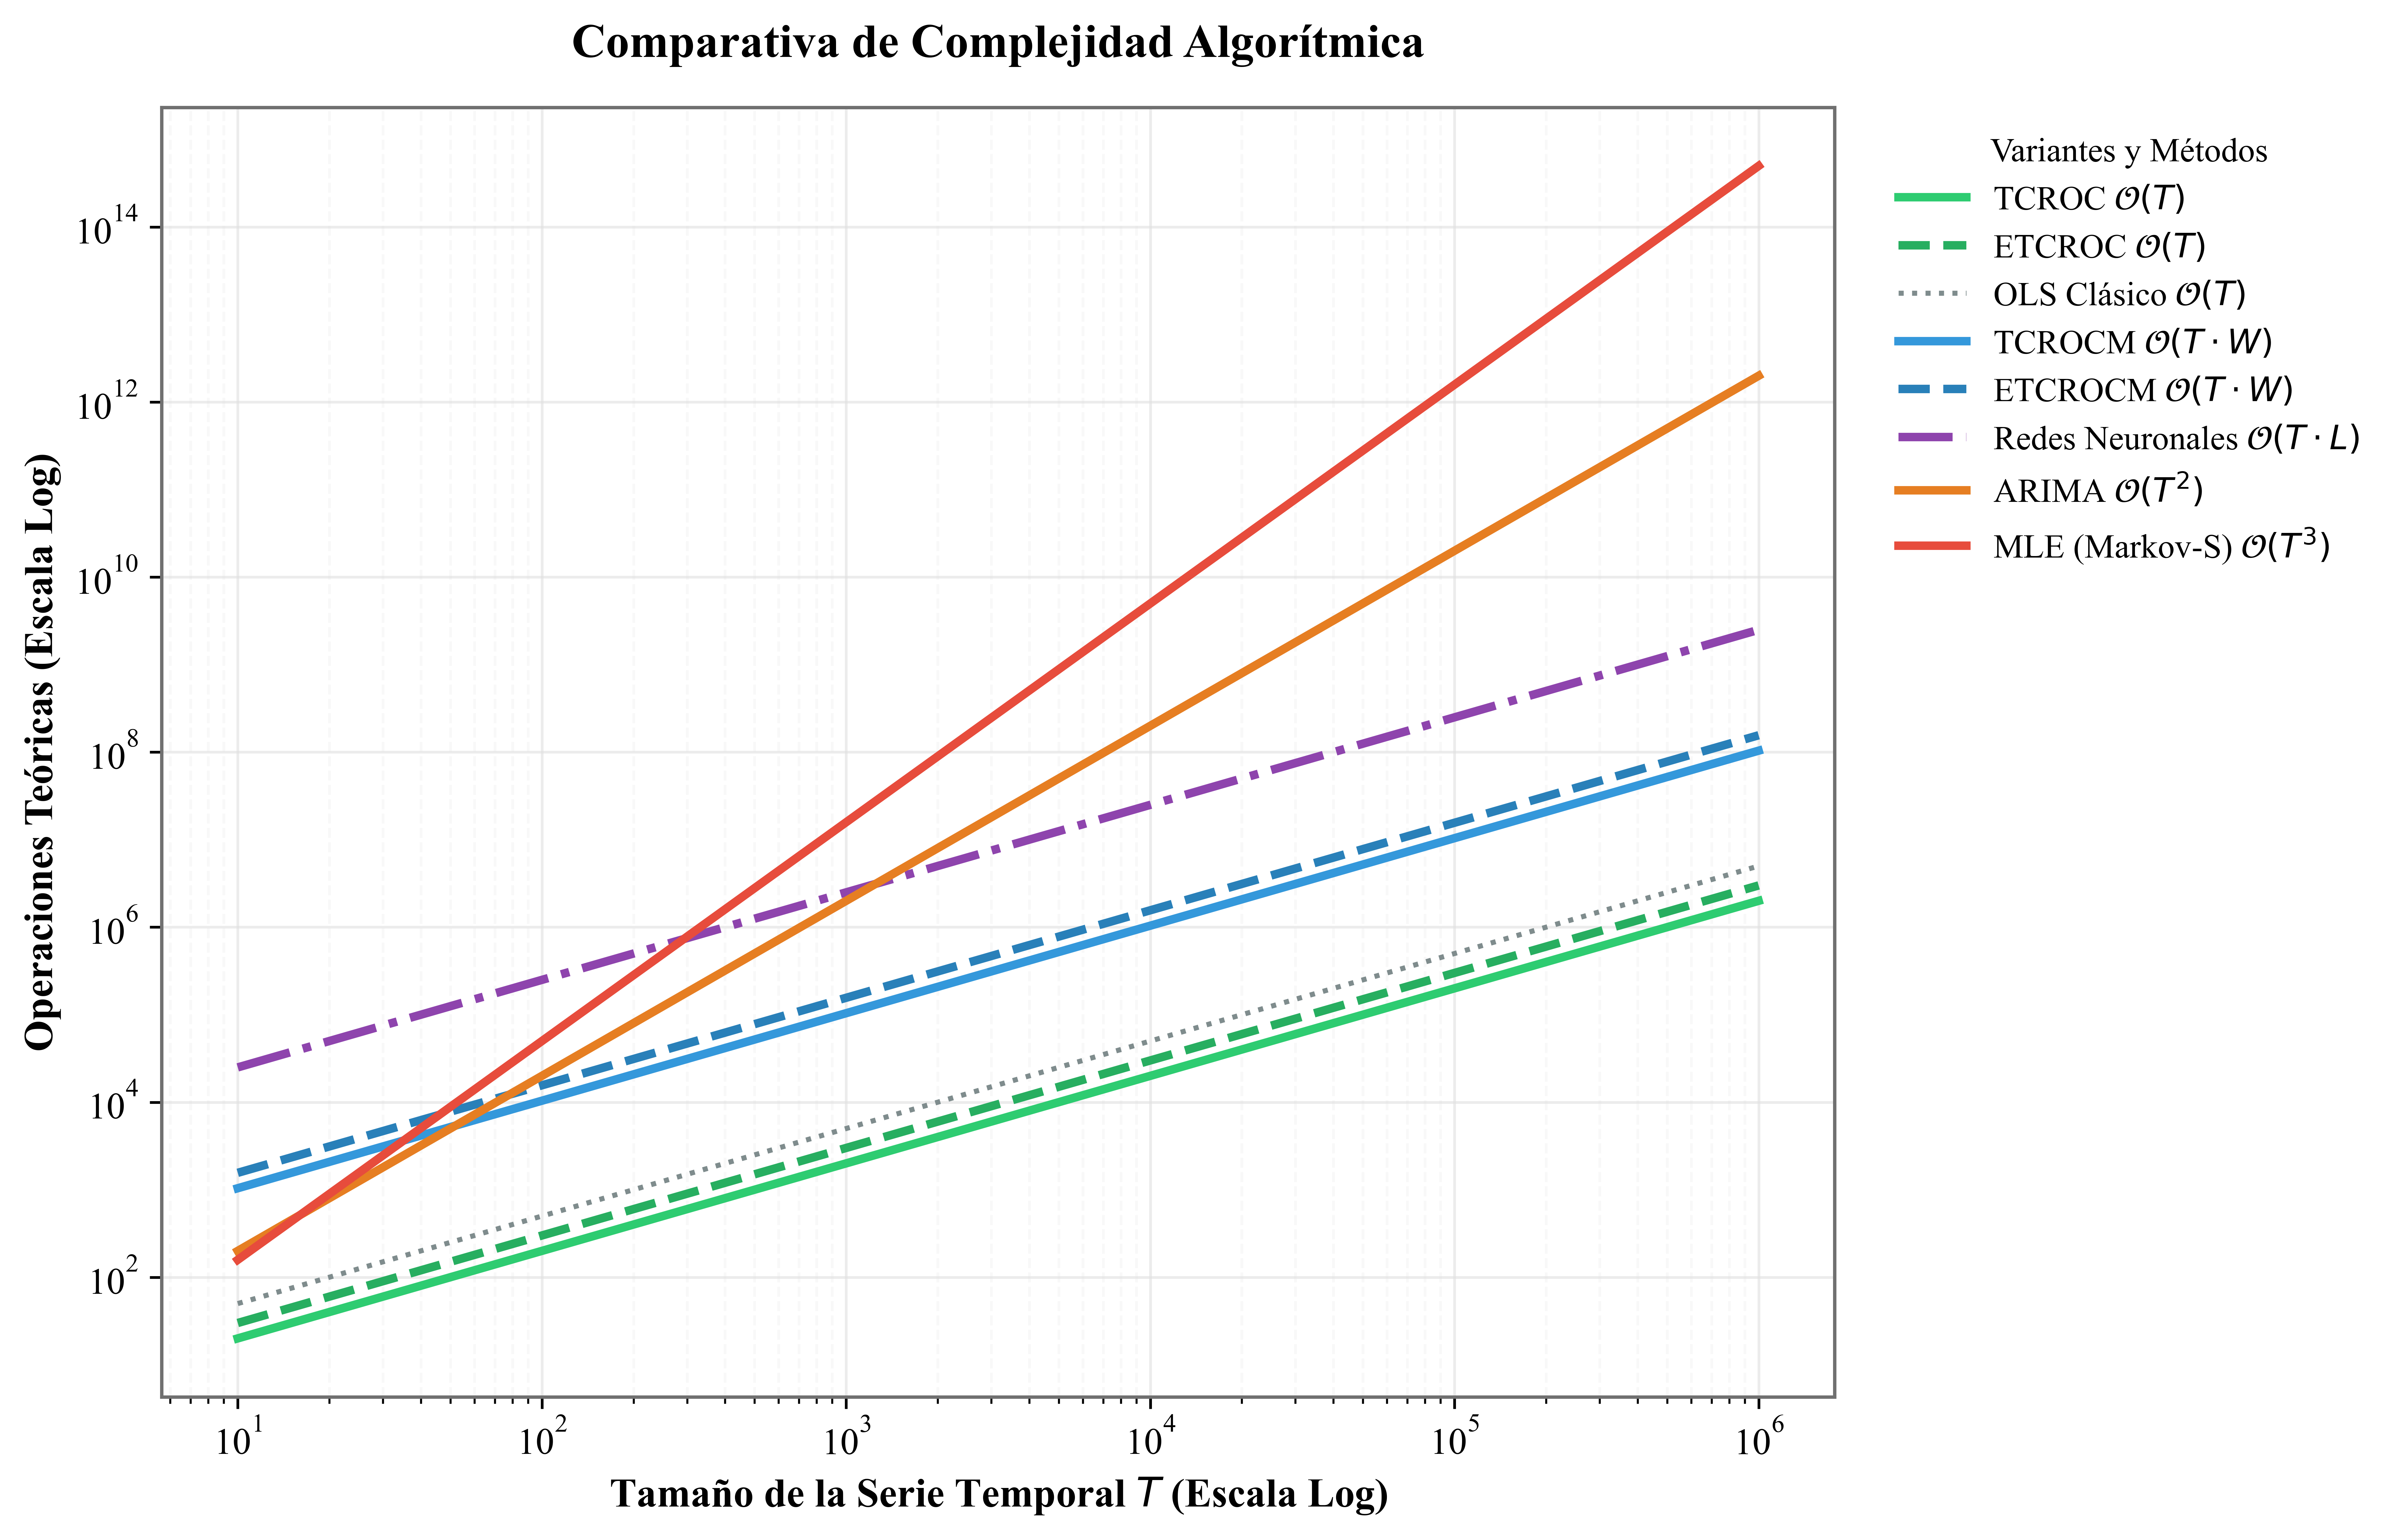
\includegraphics[width=\textwidth]{figures/CompTodosMeto.png}
\caption{Comparativa de complejidad: TCROC, TCROCM, ETCROC, ETCROCM, OLS, MLE, Redes Neuronales y ARIMA.}
\label{fig:tcroc_comp_todos}
\end{figure}

% Implementación Computacional

% --- SECCIÓN: Implementación Computacional ---
\section{Implementación Computacional}
\label{sec:tcroc_implementacion}

La siguiente función unificada en Python calcula cualquier variante de la TCROC según los parámetros proporcionados:

\begin{listing}[H]
\begin{python}
import numpy as np

def compute_tcroc(v, W=None, lambd=1.0):
    """
    Operador unificado matemáticamente eficiente para la familia TCROC.
    Calcula el escalar beta y el mapeo proyectivo alpha bajo el marco L^2.

    Parámetros
    ----------
    v : array_like (Longitud T+1)
        Vector secuencia de observaciones temporales.
    W : int, opcional
        Tamaño de la ventana (truncamiento de memoria). Si es None, W = T.
    lambd : float, opcional
        Factor amnésico de decaimiento en (0, 1]. Default: 1.0.

    Retorna
    -------
    alpha (float): Tasa de cambio relativa proyectada.
    beta (float): Factor inercial multiplicativo óptimo.
    """
    v = np.asarray(v, dtype=float)
    T = len(v) - 1
    
    # Axioma 1: Restricción Local
    if W is None or W > T:
        W = T
    elif W < 1:
        raise ValueError("La ventana local W debe ser >= 1.")

    start = T - W + 1
    v_target = v[start : T+1]
    v_lag    = v[start-1 : T]

    # Vectorización absoluta del decaimiento L^2 (evita bucles for lentos)
    # Secuencia de pesos: [lambda^(W-1), lambda^(W-2), ..., 1]
    weights = lambd ** np.arange(W - 1, -1, -1) if lambd != 1.0 else 1.0

    # Axioma 3: Solución de Mínimos Cuadrados Ponderados (Dot products en C)
    num = np.sum(weights * v_target * v_lag)
    den = np.sum(weights * (v_lag ** 2))

    if den == 0:
        raise ValueError("Degeneración algebraica: Varianza rezagada nula.")

    beta = num / den
    alpha = beta - 1.0
    
    return alpha, beta
\end{python}
\caption{Función unificada en Python para calcular las variantes de la TCROC.}
\label{lst:tcroc_implementacion}
\end{listing}

% Ejemplos Numéricos

% --- SECCIÓN: Ejemplos Numéricos Sectoriales (Perspectiva a 2026) ---
\section[Ejemplos Numéricos Sectoriales]{Ejemplos Numéricos Sectoriales (Perspectiva a 2026)}
\label{sec:tcroc_ejemplos}

Para validar empíricamente la asimilación matemática del operador, se aplica la familia TCROC sobre la macro-dimensión del \textbf{PIB en Dólares Corrientes} de la República de Honduras (periodo 2000--2024, con \(T = 24\) intervalos o transiciones observadas). Se estiman las proyecciones resultantes bajo los cuatro esquemas de asimilación paramétrica estudiados para los años fiscales 2025 y 2026.

\begin{examplex}[Proyecciones del PIB Corriente - Variante Base y Extensiones]
\label{ex:pib_dolares_2026}
Sea la secuencia empírica del PIB en dólares corrientes (millones USD) cerrando el año fiscal 2024 con un valor histórico auditado de \(37,093.57\) millones USD. 

Bajo la \textbf{TCROC global (\(W=T, \lambda=1\))}, el sumatorio agnóstico completo hereda una inercia constante \(\hat{\beta} \approx 1.0704\), indicando una tasa de asimilación proyectiva estricta de \(\alpha_T \approx 7.04\%\). 

No obstante, las perturbaciones dinámicas recientes se capturan de forma asimétrica permitiendo el ajuste de memoria y el decaimiento. En la Tabla~\ref{tab:proy_tcroc_pib}, se modelizan los escenarios inerciales divergentes según el ensamble paramétrico de pre-condicionamiento que será entregado a los agrupadores de Markov.

\begin{table}[H]
\centering
\begin{tabular}{@{}lccc@{}}
\toprule
\textbf{Variante Operacional} & \textbf{Factor ($\hat{\beta}$)} & \textbf{Proyección 2025} & \textbf{Proyección 2026} \\
\midrule
TCROC ($W=T, \lambda=1.0$)   & 1.0704 & 39\,705\,618\,091 & 42\,501\,605\,647 \\
TCROCM ($W=5, \lambda=1.0$)   & 1.0854 & 40\,259\,773\,808 & 43\,696\,240\,837 \\
ETCROC ($W=T, \lambda=0.9$)  & 1.0754 & 39\,891\,586\,807 & 42\,900\,666\,499 \\
ETCROCM ($W=5, \lambda=0.9$) & 1.0876 & 40\,343\,437\,674 & 43\,878\,039\,921 \\
\bottomrule
\end{tabular}
\caption{Modelación paramétrica divergente del PIB de Honduras (millones USD) para los años 2025--2026 bajo las cuatro formulaciones de la TCROC.}
\label{tab:proy_tcroc_pib}
\end{table}
\end{examplex}

\begin{figure}[H]
\centering
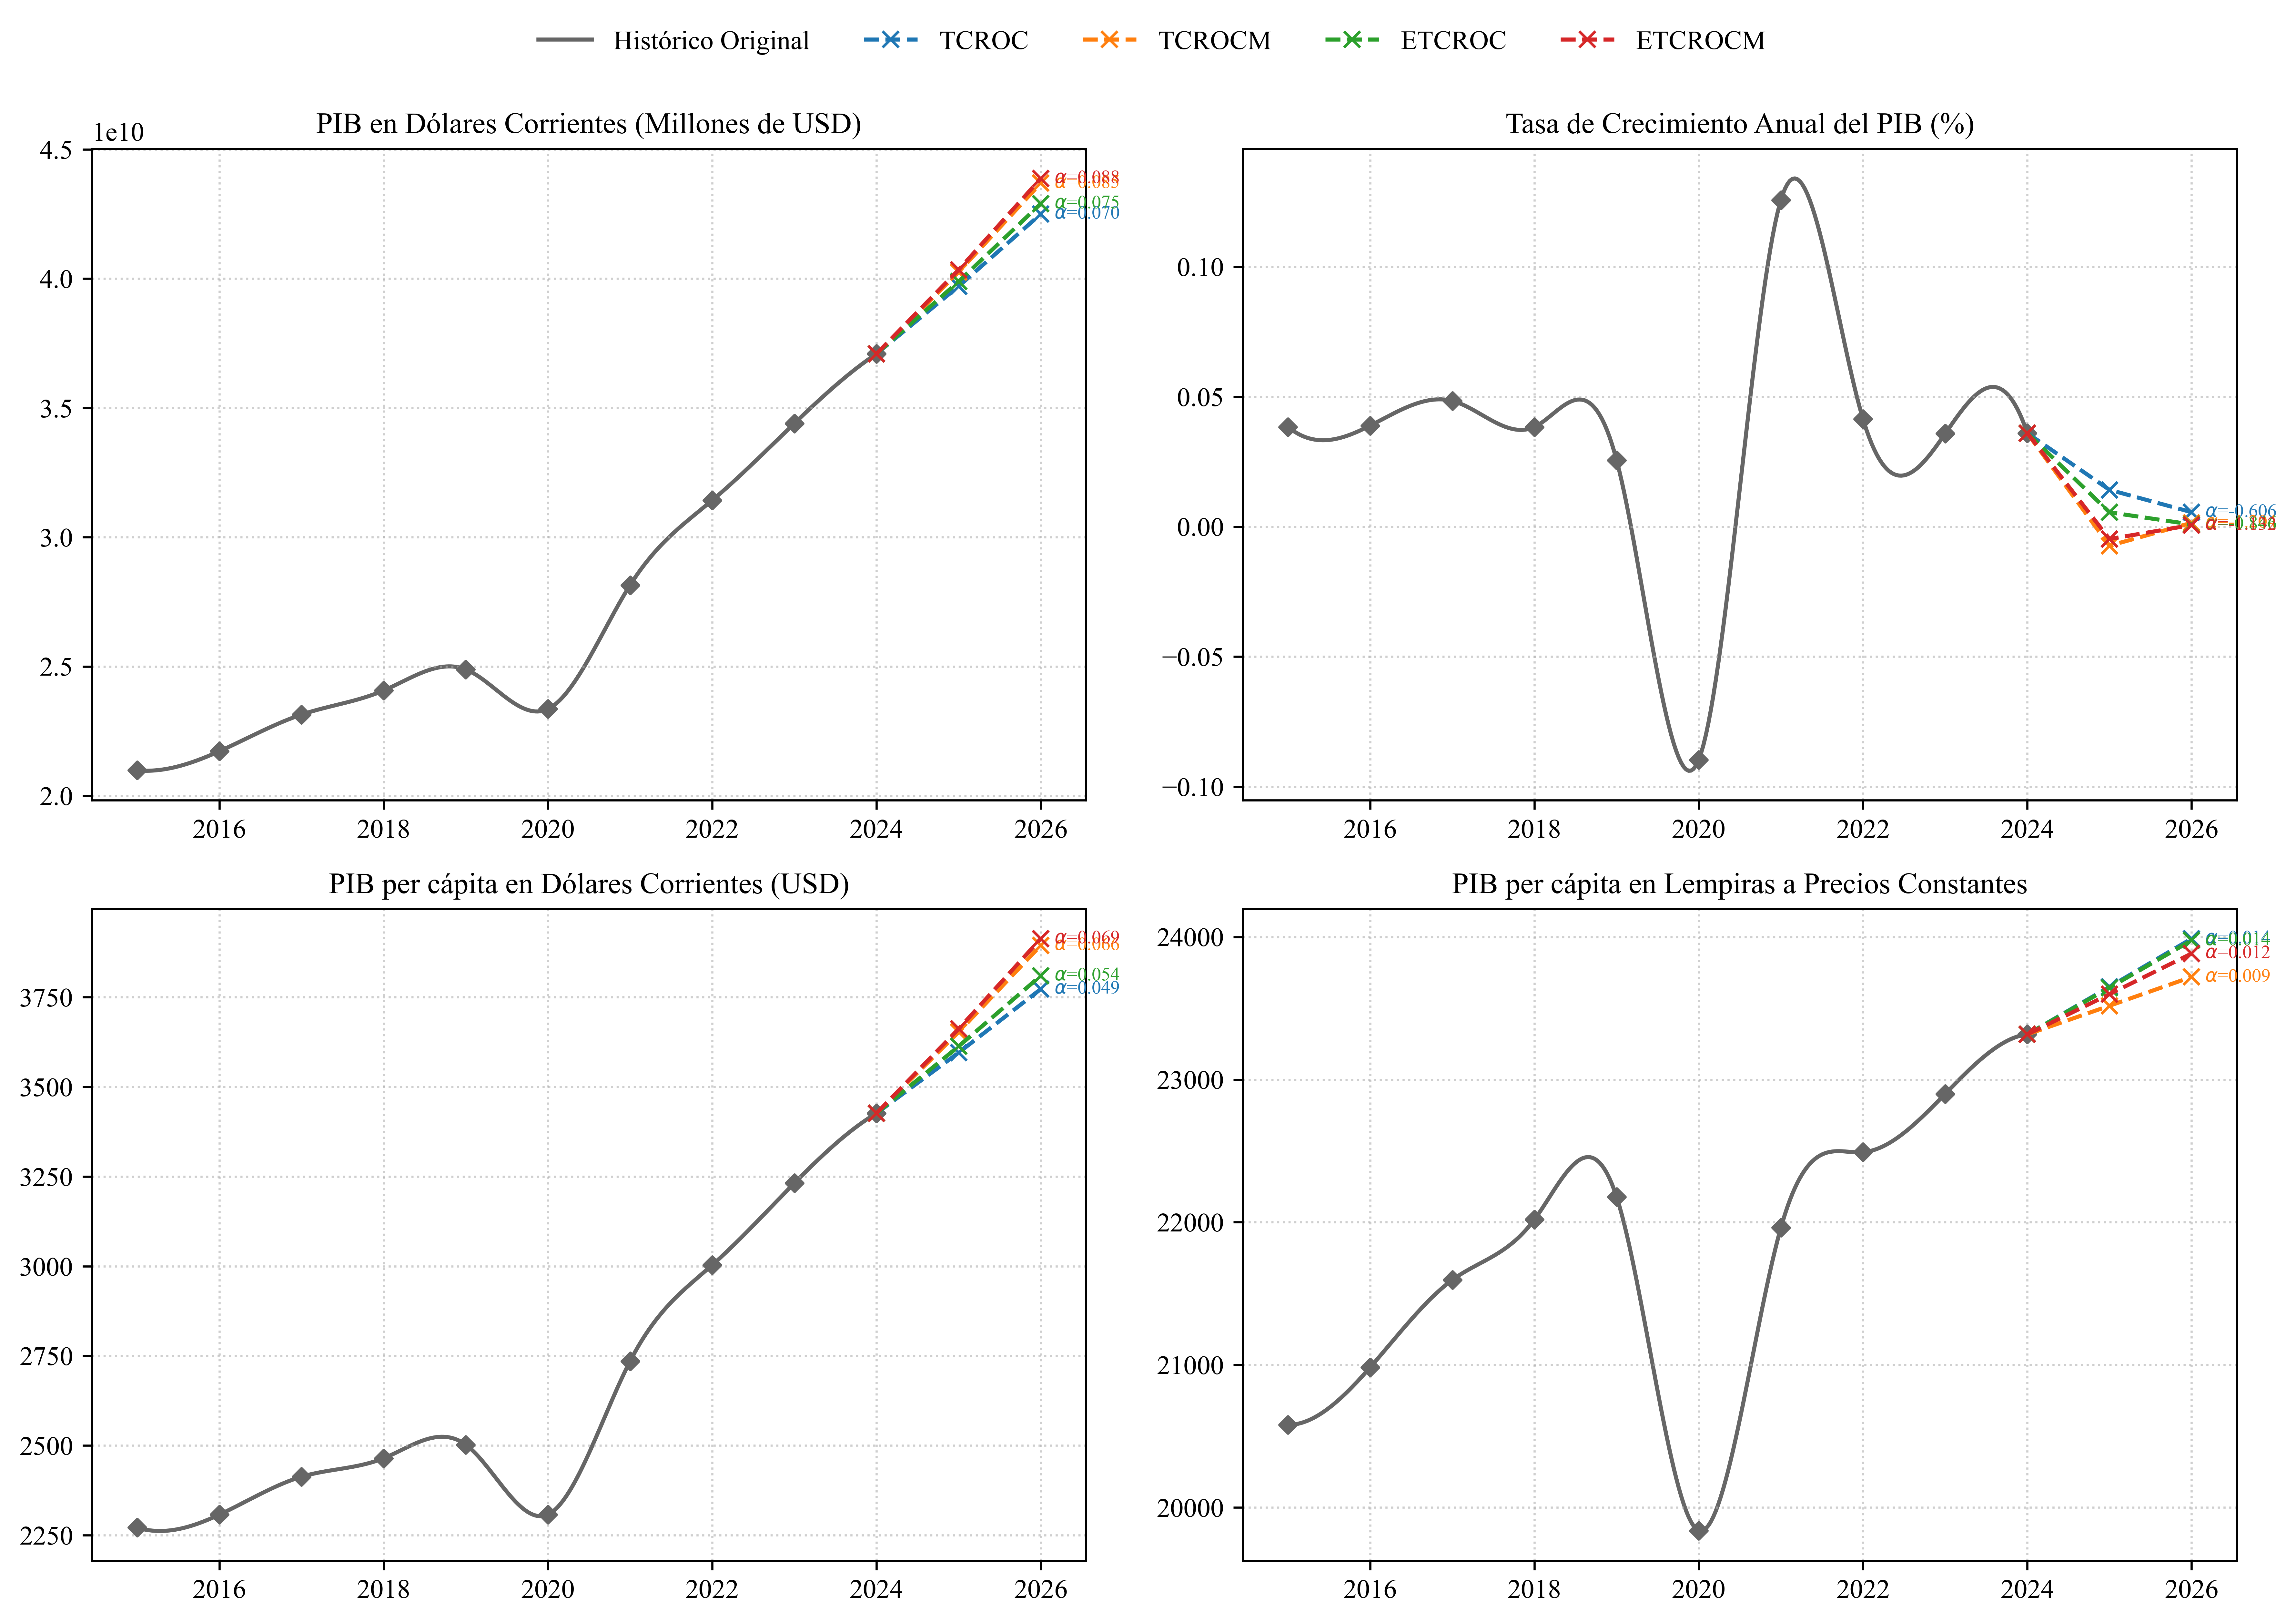
\includegraphics[width=\textwidth]{figures/EjemploPIB_TCROC_4Variantes.png}
\caption{Comparativa del espacio vectorial de entrenamiento (2000-2024) y bifurcación predictiva (2025-2026) según la asimilación del filtro TCROC para los cuatro macro-indicadores del PIB Hondureño.}
\label{fig:pib_tcroc_grid}
\end{figure}

% --- SUBSECCIÓN: Validación Cruzada Expansiva en Mercado de Combustibles --- - - - - - - - - - - - - - - - - - - - - - - - - - - - - - -
\subsection{Validación Cruzada Expansiva en Mercado de Combustibles}
\label{sec:tcroc_cv_combustibles}

Para someter el operador algorítmico al estrés provocado por los choques exógenos y volatilidades típicas del mercado energético local e internacional, se implementó un riguroso protocolo empírico de validación cruzada temporal (\textit{Expanding Window Cross-Validation}). 

Considerando el vector histórico de precios (2017--2025) de las cuatro variantes de refinamiento (Súper, Regular, Diésel y Kerosene), la partición del espacio en entrenamiento/prueba se estructuró a través de ocho anclajes temporales expansivos con un horizonte secuencial de \textit{uno-paso-adelante}:
\[
\mathcal{P} = \{60/40, 65/35, 70/30, 75/25, 80/20, 85/15, 90/10, 95/5\}
\]
donde el primer valor representa el radio de inercia in-sample y el segundo la frontera out-of-sample. Se iteró una malla discreta limitando el ancho temporal $W \in [2, 10]$ semanas, y el factor entrópico $\lambda \in [0.70, 1.00]$, calculando el desempeño de la métrica por barrido empírico general (Tabla~\ref{tab:cv_combustibles_tcroc}).

\begin{table}[H]
\centering
\resizebox{\textwidth}{!}{
\begin{tabular}{@{}lccccccccc@{}}
\toprule
& \multicolumn{8}{c}{\textbf{Desempeño MAPE (\%) por Partición Expansiva}} & \\
\cmidrule(lr){2-9}
\textbf{Macro-Serie} & \textbf{60/40} & \textbf{65/35} & \textbf{70/30} & \textbf{75/25} & \textbf{80/20} & \textbf{85/15} & \textbf{90/10} & \textbf{95/5} & \textbf{Promedio Global} \\
\midrule
\textbf{Super} & 0.71\% & 0.67\% & 0.60\% & 0.53\% & 0.50\% & 0.52\% & 0.53\% & 0.53\% & \textbf{0.57\%} \\
\textbf{Regular} & 0.70\% & 0.66\% & 0.61\% & 0.57\% & 0.48\% & 0.47\% & 0.51\% & 0.48\% & \textbf{0.56\%} \\
\textbf{Diesel} & 0.80\% & 0.77\% & 0.65\% & 0.62\% & 0.62\% & 0.58\% & 0.60\% & 0.56\% & \textbf{0.65\%} \\
\textbf{Kerosene} & 1.07\% & 0.99\% & 0.90\% & 0.80\% & 0.80\% & 0.78\% & 0.82\% & 0.83\% & \textbf{0.87\%} \\
\bottomrule
\end{tabular}
}
\caption{Evolución del error predictivo porcentual absoluto (MAPE) a lo largo de los anclajes temporales de validación un-paso-adelante para los cuatro macro-indicadores energéticos.}
\label{tab:cv_combustibles_tcroc}
\end{table}

De la evidencia tabulada resulta revelador observar cómo el ajuste dinámico absoluto del mercado de hidrocarburos demanda siempre un truncamiento de la ventana de arrastre a \(W=2\). Esto demuestra matemáticamente el postulado heurístico de hiper-reactividad a corto plazo en las bolsas de combustibles: la volatilidad reciente anula por completo la relevancia explicativa del pasado remoto (el cual actúa puramente como ruido estocástico perjudicial para el pronóstico un-paso-adelante).

% Relación con Métodos Establecidos

% --- SECCIÓN: Relación con Métodos Establecidos ---
\section{Relación con Métodos Establecidos}
\label{sec:tcroc_relacion}

La familia TCROC comparte fundamentos con métodos clásicos de análisis de series temporales. A continuación se resumen las principales comparaciones.

\textbf{TCROC vs.\ Mínimos Cuadrados Ordinarios.} Ambos minimizan la suma de cuadrados. La TCROC se especializa en la relación \(v(t) \approx \hat{\beta}\,v(t-1)\), ofreciendo una interpretación directa como tasa de cambio relativa, con idéntica complejidad \(\mathcal{O}(T)\).

\textbf{TCROC vs.\ Modelos ARIMA.} Un modelo AR(1) sin intercepto, \(v(t) = \phi\,v(t-1) + \varepsilon(t)\), produce el mismo estimador OLS que la TCROC, con \(\alpha_T = \hat{\phi} - 1\). Sin embargo, ARIMA generaliza a órdenes superiores (AR($p$), MA($q$), diferenciación), capturando estacionalidad y retardos múltiples a costa de mayor complejidad \(\mathcal{O}(T^2)\) \cite{Box2015}.

\textbf{TCROC vs.\ Estimación de Máxima Verosimilitud.} MLE asume un marco probabilístico (e.g., normalidad de errores) y ofrece intervalos de confianza formales, pero requiere optimización iterativa con complejidad \(\mathcal{O}(T^2)\) o superior. La TCROC, sin supuestos distribucionales explícitos, proporciona una solución analítica cerrada \cite{Greene2018}.

\textbf{ETCROC y ETCROCM vs.\ GLS.} Como se demostró en el Teorema~\ref{teo:optimalidad_general}, las variantes con decaimiento exponencial coinciden con estimadores GLS bajo estructuras de covarianza proporcionales a \(\lambda^{-(T-t)}\), lo que las posiciona como casos particulares de la teoría de mínimos cuadrados generalizados.

\textbf{TCROCM y ETCROCM vs.\ Modelos con ventanas.} El enfoque de ventana móvil es análogo al utilizado en medias móviles y filtros adaptativos, pero la familia TCROC optimiza un factor multiplicativo en lugar de un promedio aritmético, preservando la interpretación como tasa de cambio relativa.

% Conclusiones

% --- SECCIÓN: Conclusiones ---
\section{Conclusiones}
\label{sec:tcroc_conclusiones}

En este capítulo se ha desarrollado la familia de métodos TCROC para el modelado de series temporales económicas y financieras, compuesta por cuatro variantes jerárquicamente relacionadas. Las principales contribuciones son:

\begin{enumerate}
    \item Se estableció un \textbf{marco general unificado} (ecuación~\ref{eq:tcroc_general}) del cual TCROC, TCROCM, ETCROC y ETCROCM se derivan como casos particulares, controlados por los parámetros $\lambda$ y $W$.

    \item Se demostraron rigurosamente las propiedades de \textbf{existencia y unicidad} del estimador $\hat{\beta}$ para todas las variantes, basándose en la convexidad estricta de la función objetivo cuadrática.

    \item Se probó la \textbf{consistencia asintótica} de los estimadores bajo modelos AR(1) estacionarios, la \textbf{continuidad} respecto a perturbaciones paramétricas, la \textbf{estabilidad} frente a perturbaciones acotadas (con cotas de tipo Lipschitz), y la \textbf{optimalidad} en el sentido de Gauss-Markov (OLS para TCROC/TCROCM, GLS para ETCROC/ETCROCM).

    \item Se analizó la \textbf{complejidad computacional}, que oscila entre \(\mathcal{O}(T)\) para TCROC y ETCROC, y \(\mathcal{O}(T \cdot W)\) para las variantes con ventana móvil, siendo en todos los casos inferior a la de ARIMA.

    \item Se proporcionó una \textbf{implementación computacional unificada} y ejemplos numéricos con datos del PIB de Honduras, que ilustran la aplicabilidad del método y su capacidad de pronóstico.
\end{enumerate}

No obstante, las variantes presentadas se restringen a relaciones lineales y son sensibles a valores atípicos. La integración de técnicas de robustez (estimadores M, funciones de influencia) y la incorporación de componentes estocásticos más complejos constituyen líneas de desarrollo futuro. En el capítulo siguiente se abordará la \textbf{TCROC-Markov}, que introduce dependencias de régimen mediante cadenas de Markov para capturar cambios estructurales en la dinámica de la serie.

% -------------------------------------------------------------------
% -------------------------------------------------------------------
% CAPÍTULO
% -------------------------------------------------------------------
